\documentclass{article}


\usepackage[utf8]{inputenc}
\usepackage[english]{babel}
\usepackage{amsmath}
\usepackage{amssymb}
\usepackage{todonotes}
\usepackage{mathrsfs}
\usepackage{mathtools}
\usepackage{xcolor}
\usepackage{url}
\usepackage[nottoc,notlot,notlof]{tocbibind}

\usepackage{natbib}
\bibliographystyle{abbrv}

\usepackage{tikz}
\usetikzlibrary{arrows}

\usepackage{listings}
\usepackage{courier}

\lstset{basicstyle=\footnotesize\ttfamily,breaklines=true}
\lstset{framextopmargin=50pt}

\newcommand{\RN}[1]{%
  \textup{\uppercase\expandafter{\romannumeral#1}}%
}

\newcommand{\figref}[1]{\figurename~\ref{#1}}

\title{PyPropagate \\ A Python Framework for stationary paraxial wave propagation}
\author{Lars Melchior }
\date{\today}

\begin{document}
\maketitle
\clearpage
\tableofcontents
\clearpage

\section{Introduction}

\clearpage

\section{Theory}


\subsection{The Paraxial Wave Equation}

\subsubsection{Complex Amplitude} \label{sec:phasors}

A plane wave $\phi$ traveling in $z$ direction with amplitude $A$, phase speed $v$ and frequency $\omega$ can be mathematically expressed as

\begin{align} \label{eq:plane_wave}
\phi = A \sin(\omega \cdot (z/v - t) ).
\end{align}

Electromagnetic waves in vacuum have the phase speed $v = c$, where $c$ is the speed of light. In a medium these waves are slowed down by a factor $n$, which is the refractive index of the medium $v = c/n$. Additionally, the wave Amplitude falls exponentially from an initial Value $A_0$ with the penetration depth $z$ and linear attenuation coefficient $\mu$ of the medium $A = A_0 \cdot \exp(- \mu z)$. Using Euler's formula $\exp(ix) = \cos(x) + i \sin(x)$ the refractive index and the linear attenuation coefficient can be combined into the \emph{complex refractive index} $\underline n = n + i \mu  / k$ with the wave number $k = \omega/c$. Using this we can rewrite equation~\eqref{eq:plane_wave} as

\begin{align*}
\phi = \Im \mathopen{} \left( A_0 \cdot e^{ i (\underline n k z - \omega t) } \right) \mathclose{},
\end{align*}

where $\Im$ denotes the imaginary part. We will refer to the argument of $\Im$ as the \emph{phasor} representation of $\phi$. If $\phi$ describes the amplitude of a monochromatic and linear polarized electromagnetic wave, we call the argument of $\Im$ the \emph{complex amplitude} $\psi$ of the wave. The complex amplitude is connected to the local intensity $I$ of the wave through the relationship~\cite{wiki:intensity}

\begin{align*}
I = \frac{c n \epsilon_0}{2} |\psi|^2,
\end{align*}

where $\epsilon_0 \approx 8.854 \cdot 10^{-12} F/m$ is the vacuum permittivity.


\subsubsection{Propagation of electromagnetic waves in matter}

The dynamics of electromagnetic waves are governed by Maxwell's Equations~\cite{PriciplesOfOptics}. For a monochromatic wave in a homogeneous, linear, and isotropic dielectric medium without free charges they take the form

\begin{eqnarray*}
\vec \nabla \vec E = 0 && \vec \nabla \times \vec E = - \frac{ \partial \vec B }{ \partial t }  \\
\vec \nabla \vec B = 0 && \vec \nabla \times \vec B = \frac{n^2}{c^2} \frac{ \partial \vec E }{ \partial t },
\end{eqnarray*}

where $\vec B$ is the magnetic field vector, $\vec E$ is the electric field vector, $c$ is the speed of light in vacuum and $n$ is the refractive index of the medium. Note that $n$ is usually dependent on the frequency $\omega$ of the wave. We can include the effects of absorption at any point by using the phasor representation for the fields and replacing $n$ with the complex refractive index $\underline n$. Using the curl of the curl identity $\vec \nabla \times \vec \nabla \times \vec E = \vec \nabla (\vec \nabla  \vec E ) - \Delta  \vec E$ we obtain a wave equation for the electric field

\begin{align} \label{eq:wave_equation} 
\frac{n^2}{c^2} \frac{ \partial^2 \vec E }{ \partial t^2 } & = \Delta \vec E.
\end{align}

Analogously we find the same wave equation for the magnetic field. Since the divergence of $\vec E$ and $\vec B$ is zero, only transverse waves are possible as longitudinal waves would describe wells and sinks in the field. Since the time derivative of the dot product of $\vec E$ and $\vec B$ disappears, we can see that the electric field oscillates orthogonally to the magnetic field. We apply above equations on a medium with piecewise constant $n$ by requiring continuity of the fields. Since the wave equation \eqref{eq:wave_equation} is linear, solutions can be written as superpositions of linear polarized waves $\vec E = \vec{e}_i \, \psi $, where $\vec{e}_i$ is the unit vector in direction of polarization and $\psi$ is the amplitude.

\subsubsection{Stationary solutions}

We now regard stationary solutions to the wave equation where the intensity remains unchanged in time. Mathematically, $\psi$ separates into the product of a spatially and a temporally dependant part $\psi = \psi_t(t) \cdot \psi_{\vec x}(\vec x)$. After substituting this into equation \eqref{eq:wave_equation} and reordering terms we get

\begin{align}  \label{eq:stationary_1}
\frac{1}{\psi_t} \frac{ \partial^2 \psi_t }{ \partial t^2 } & = \frac{c^2}{n^2 \psi_{\vec x}} \Delta \psi_{\vec x}.
\end{align}

The left side of the equation does not contain any terms that depend on location and the right side does not contain any that depend on time. Therefore neither side can be dependent of time or location and is equal to a constant value. The ansatz $\psi_t = \sin(\omega t)$ gives us

\begin{align*} 
\frac{1}{\psi_t} \frac{ \partial^2 \psi_t }{ \partial t^2 } = -\omega^2. 
\end{align*}

Substituting this into equation \eqref{eq:stationary_1} and reordering terms yields

\begin{align} \label{eq:helmholtz}
\Delta \psi_{\vec{x}} + n^2 k^2 \psi_{\vec{x}} & = 0,
\end{align}

where $k = \omega / c$ is the wave number. This is the Helmholtz Equation \cite{PriciplesOfOptics}.


\subsubsection{Paraxial Approximation} \label{sec:paraxial_equation}

We now look for solutions of the Helmholtz Equation which represent waves traveling in $z$ direction or at a small angle to the $\vec{e}_z$ axis. We can write these solutions as $\psi_{\vec{x}} = u(x,y,z) \cdot \exp(i k z)$ with a complex envelope $u(x,y,z)$ that changes slowly in $z$ direction. Particularly,

\begin{align*}
\left| \frac{\partial^2 u}{\partial z^2} \right| \ll \left|  k \frac{\partial u}{\partial z}  \right|.
\end{align*}

Inserting this into equation \eqref{eq:helmholtz} and neglecting very small terms gives us:

\begin{align*}
2 i k \frac{\partial u}{\partial z} + \frac{\partial^2 u}{\partial x^2} + \frac{\partial^2 u}{\partial y^2} + k^2 (n^2 - 1) u = 0.
\end{align*}

For convenience we define $A := \frac{i}{2k}$ and $F := \frac{ik}{2} (n^2 - 1) $ which let us write the partial differential equation more concisely as

\begin{align} \label{eq:paraxial_wave_equation}
\frac{\partial u}{\partial z} = A \left( \frac{\partial^2 u}{\partial x^2} + \frac{\partial^2 u}{\partial y^2} \right) + F  u,
\end{align}

which is known as the paraxial wave equation.

\clearpage

\subsection{Fresnel Diffraction Integral}

For constant $F$ we find an elementary solution to the paraxial wave equation

\begin{align*}
\mathcal{U}(x,y,z) = \frac{1}{4 \pi A z} \, \exp \! \left(F z-\frac{1}{4 A z} \; (x^2+y^2)\right),
\end{align*}

which can be verified by insertion. We show that $\lim_{z \rightarrow 0} \mathcal{U}(x,y,z) = \delta(x)\delta(y)$ where $\delta(x)$ is the Dirac delta distribution. First we define $g_z(x) := \exp(-x^2/4 A z) /$ $\sqrt{4 \pi A z}$. Then, for any bounded contiguous function $f$,

\begin{align*}
    \lim_{z \rightarrow 0} \int_\mathbb{R} f(x) \, g_z(x)  \; \text{d}x & = 
    \lim_{z \rightarrow 0} \frac{1}{\sqrt{A \pi}} \int_\mathbb{R} f(\sqrt{4 z} \, u) \, \exp(-u^2/A)  \; \text{d}u \\
    & =  \frac{1}{\sqrt{A \pi}} \int_\mathbb{R} f(0) \, \exp(-u^2/A)  \; \text{d}u \\
    & = f(0) = \int_\mathbb{R} f(x) \, \delta(x)  \; \text{d}x,
\end{align*}

where we used the monotone convergence theorem in third third step. This result implies weak convergence $g_z \! \xrightarrow[]{w} \! \delta$. The claim follows analogously for $\lim_{z \rightarrow 0} $ $ \mathcal{U}(x,y,z) = \lim_{z \rightarrow 0} \exp(Fz) g_z(x) g_z(y)$. Since equation \eqref{eq:paraxial_wave_equation} is linear and translation invariant, we can use this property to obtain a solution for any boundary condition $u(x,y,0)$ at $z = 0$

\begin{align*}
u(x,y,z) = \iint_{-\infty}^{+\infty} u(x,y,0) \cdot \, \mathcal{U}(x-x',y-y', z) \; \mathrm d x' \mathrm d y'.
\end{align*}

This can be more compactly expressed through a 2D convolution:

\begin{align} \label{eq:fresnel_convolution}
u(x,y,z) =  u(x,y,0) * \mathcal{U}(x,y,z).
\end{align}


\clearpage

\section{Propagators}
\subsection{Field Discretization}

\label{sec:discretization}

\begin{figure}[!ht]
  \centering
  
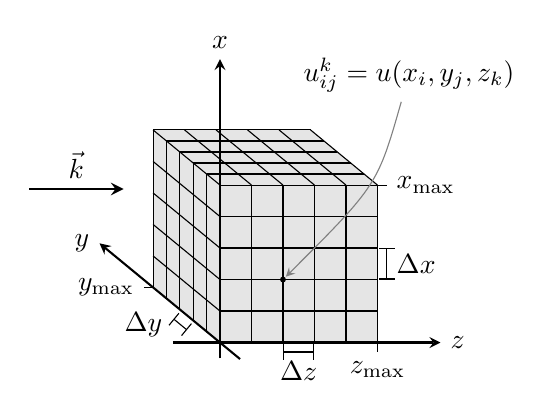
\begin{tikzpicture}[x={(0.0cm,0.4cm)},y={(-0.17cm,0.14cm)},z={(0.4cm,0.0cm)},>=stealth]

% box fill
\def\sidelength{5}

\fill[black!10] (xyz cs:x=0) -- (xyz cs:y=\sidelength) -- (xyz cs:x=\sidelength,y=\sidelength)  -- (xyz cs:x=\sidelength,y=\sidelength,z=\sidelength)  -- (xyz cs:x=\sidelength,z=\sidelength) -- (xyz cs:z=\sidelength);

% box grid
\foreach \coo in {1,2,...,\sidelength}{
  \draw (xyz cs:x=\coo) -- (xyz cs:z=\sidelength,x=\coo);
  \draw (xyz cs:x=\coo) -- (xyz cs:y=\sidelength,x=\coo);

  \draw (xyz cs:y=\coo) -- (xyz cs:x=\sidelength,y=\coo);
  \draw (xyz cs:y=\coo,x=\sidelength) -- (xyz cs:x=\sidelength,z=\sidelength,y=\coo);

  \draw (xyz cs:z=\coo) -- (xyz cs:x=\sidelength,z=\coo);
  \draw (xyz cs:z=\coo,x=\sidelength) -- (xyz cs:x=\sidelength,y=\sidelength,z=\coo);
}

% axes
\draw[line width=0.75pt,->] (xyz cs:x=-0.5) -- (xyz cs:x={\sidelength+4}) node[above] {$x$} ;
\draw[line width=0.75pt,->] (xyz cs:y=-1.5) -- (xyz cs:y={\sidelength+4}) node[left] {$y$};
\draw[line width=0.75pt,->] (xyz cs:z=-1.5) -- (xyz cs:z={\sidelength+2}) node[right] {$z$};

\draw [arrows={|-|}] (xyz cs:z={\sidelength+0.3pt},x=2) -- node[right] {$\Delta x$} (xyz cs:z={\sidelength+0.3pt},x=3);
\draw [|-|] (xyz cs:x=-0.3pt,y=2,z=-0.2pt) -- node[left = 3pt] {$\Delta y$} (xyz cs:x=-0.3pt,y=3,z=-0.2pt);
\draw [|-|] (xyz cs:x=-0.3pt,z=2) -- node[below] {$\Delta z$} (xyz cs:x=-0.3pt,z=3);

\draw (xyz cs:y=\sidelength) -- (xyz cs:y=\sidelength,z=-0.3pt) node[left] {$y_\mathrm{max}$};
\draw (xyz cs:x=\sidelength,z=\sidelength) -- (xyz cs:x=\sidelength,z={\sidelength+0.3pt}) node[right] {$x_\mathrm{max}$};
\draw (xyz cs:z=\sidelength) -- (xyz cs:x=-0.3pt,z={\sidelength}) node[below] {$z_\mathrm{max}$};

\draw [line width=1pt,->] (xyz cs:x=4,y=2.5,z=-5) -- node[above] {$\vec{k}$} (xyz cs:x=4,y=2.5,z=-2) ; 

\node[fill,circle,inner sep=0.75pt] at (2,0,2) {};

\node[align=center] at (8.5,0,6) (ori) {$u_{ij}^k = u(x_i,y_j,z_k)$};
\draw[->,color=gray,shorten >=1.5pt] (ori) .. controls (5,0,5)  .. (2,0,2);

\end{tikzpicture}

  \caption{We discretize the complex envelope into an euclidean grid of equidistantly spaced coordinates $x_i$, $y_j$, $z_k$ in the respective directions. Here each axis is split into $N_x = N_y = N_z = 6$ segments and begins at $x_\mathrm{min} = y_\mathrm{min} = z_\mathrm{min} = 0$. In the paraxial approximation the wave vector $\vec k$ is approximately parallel to the $z$ axis.}
\end{figure}


We now consider the complex envelope at discretized coordinate positions

\begin{align*}
u(x,y,z) \rightarrow u(x_i,y_j,z_k) := u_{i,j}^k,
\end{align*}

for $i \in \{0..N_x-1\}$ and $N_x$ equally distributed points  $x_i \in [x_\mathrm{min},x_\mathrm{max}]$ with distance $\Delta x = (x_\mathrm{max} - x_\mathrm{min})/(N_x-1)$. The definitions are analogous for $y_j$ and $z_k$.

If the field is assumed to be constant in $y$ direction, we can drop the explicit $y$ dependence, resulting in the 2D field:

\begin{align*}
u(x,y,z) = u(x,0,z) \rightarrow u(x_i,0,z_k) := u_{i}^k.
\end{align*}

 If the field $u_{i,j}^k$ for a given $k$ is known, we use a propagator to calculate the field at the next discretized $z$ value according to the the paraxial wave equation \eqref{eq:paraxial_wave_equation} and some boundary condition. We define the convenience variables $n_x = N_x - 2$ and $n_y = N_y - 2$.
 
\clearpage

\subsection{Fresnel Propagator \label{sec:fresnel_propagator}}


With equation \eqref{eq:fresnel_convolution} we derived an exact update rule for $u_{i,j}^{k} \rightarrow u_{i,j}^{k+1}$ when $F$ is constant in the interval $[z_k,z_{k+1})$. To derive an efficient algorithm we first write the convolution as a multiplication in Fourier space using the 2D Fourier transform $\mathscr{F}$ in $x$ and $y$ direction~\cite{wiki:convolution_theorem}

\begin{align} \label{eq:fresnel_fourier_convolution}
\begin{split}
u(x,y,z+\Delta z) &= u(x,y,z) * \mathcal{U}(x,y,\Delta z) \\
&= \mathscr{F}^{-1}[ \mathscr{F}[u(x,y,z)] \cdot \mathscr{F}[\mathcal{U}(x,y,\Delta z)] ].
\end{split}
\end{align}

Since $A$ is imaginary (or more importantly: $\Re(A) = 0$), the Fourier transform of $\mathcal{U}(x,y,\Delta z)$ is given by:

\begin{align*}
\mathscr{F}[\mathcal{U}(x,y,\Delta z)](k_x,k_y) = \frac{1}{2 \pi} \exp \! \left( F \Delta z - A \Delta z (k_x^2+k_y^2)\right).
\end{align*}

If we interpret the discretized field as a Dicac comb and assume periodic boundary conditions, the Fourier transform in equation \eqref{eq:fresnel_fourier_convolution} becomes the the 2D Discrete Fourier Transform (DFT) and its inverse (iDFT)~\cite{wiki:DFT}. This gives us an update rule for the field matrix $(u^k)_{i,j} = u^k_{i,j}$

\begin{align} \label{eq:fresnel_DFT}
u^{k+1} = \exp(F \Delta z)  \, \mathrm{iDFT} \! \left[ \mathrm{DFT} \! \left[ u^{k} \right]\!(k_x,k_y) \cdot \exp \! \left(-A \Delta z (k_x^2+k_y^2)\right) \right],
\end{align}

where the multiplications are performed element-wise with the discretized field. By calculating the DFT using a Fast Fourier Transform this step can be performed in $\mathcal{O}(n_x n_y \cdot log(n_x n_y))$ time complexity~\cite{wiki:FFT}.

Note that this formulation of the Fresnel propagator can also give an approximate solution for non constant $F$ when the step size $\Delta z$ is chosen small enough that diffraction effects in $x,y$ direction between neighboring cells are negligibly small\todo{proof if possible. Reference to multislice-paper?}.















\clearpage
 
\subsection{Finite Difference Propagator \label{sec:finite_differences_propagator}}


\subsubsection{Two Dimensions} \label{sec:finite_difference_propagator_2D}

If the field is constant in $y$ direction, equation  \eqref{eq:paraxial_wave_equation} becomes

\begin{align*}
\frac{\partial u}{\partial z} = A\frac{\partial^2 u}{\partial x^2} + F  u.
\end{align*}

Since field values are given at discretized points, we approximate derivatives with their difference quotient

\begin{align*}
\left. \frac{\partial u}{\partial z}  \right\rvert_{\substack{x=x_i\\z=z_k}} \! &\rightarrow \frac{u_i^{k+1} - u_i^{k}}{\Delta z} &
\left. \frac{\partial^2 u}{\partial x^2}  \right\rvert_{\substack{x=x_i\\z=z_k}} \! &\rightarrow \frac{u_{i-1}^{k} - 2 u_{i}^{k} + u_{i+1}^{k}}{\Delta x^2},
\end{align*}

resulting in the forward Euler step

\begin{align*}
\frac{u_i^{k+1} - u_i^{k}}{\Delta z} =
A \frac{u_{i-1}^{k} - 2 u_{i}^{k} + u_{i+1}^{k}}{\Delta x^2} + F(x_i,0,z_k) u_{i}^{k}  := f^k_i .
\end{align*}

The Euler method is only first-order accurate and is numerically unstable at large step sizes. We therefore implement our propagator using the Crank–Nicolson method, which is an implicit method that is second-order accurate in $\Delta x$ and $\Delta z$ and unconditionally stable~\cite{DissertationFuhse}

\begin{align*}
\frac{u_i^{k+1} - u_i^{k}}{\Delta z} := \frac{ f^k_i +  f^{k+1}_i }{2} .
\end{align*}

Reordering terms and introducing the auxiliary variables $r_A = A \frac{\Delta z}{ \Delta x^2}$ and $C_i^{k} = \frac{\Delta z}{2} F(x_i,0,z_{k})$ gives us

\begin{align} \label{eq:2D_finite_difference_equation}
\begin{split}
 & u_i^{k+1} ( 1 + 2 \, r_x - C_i^{k+1} ) - r_x ( u_{i-1}^{k+1} + u_{i+1}^{k+1} )\\
= \; &  u_i^{k \phantom{ + 1} } ( 1 - 2\,r_x + C_i^{k \phantom{ + 1} }) + r_x (u_{i-1}^{k \phantom{ + 1} } + u_{i+1}^{k \phantom{ + 1} }  ).
\end{split}
\end{align}

If the boundary conditions at the edges $u_0^k$ and $u_{n_x+1}^k$ are known for all $k$, equation \eqref{eq:2D_finite_difference_equation} can be rewritten as the matrix equation

\begin{align} \label{eq:FD1DMatrixEquation}
B^n \boldsymbol u^{k+1} = \boldsymbol d^k,
\end{align}

where $\left(\boldsymbol u^{k}\right)_i = u_{i}^{k}$, $B^n$ is the $n_x \times n_x$ tridiagonal matrix

\begin{align*}
B^n = \left(
\begin{matrix}
    ( 1 + 2 \, r_x - C_1^{k+1} ) & - r_x & 0 &   \\
    - r_x  & ( 1 + 2 \, r_x - C_2^{k+1} ) & - r_x  & \dots \\
    0 & - r_x  & ( 1 + 2 \, r_x - C_3^{k+1} ) &  \\
     & \vdots & & \ddots
\end{matrix}
\right),
\end{align*}

and $d^k$ is a vector containing the right side of equation \eqref{eq:2D_finite_difference_equation} and the edge boundary conditions

\begin{align*}
\boldsymbol d^k = \left(
\begin{matrix}
u_{1}^{k } ( 1 - 2\,r_x + C_1^{k}) + r_x (u_{0}^{k } + u_{2}^{k } + u_{0}^{k+1} ) \\
u_i^{k } ( 1 - 2\,r_x + C_2^{k }) + r_x (u_{1}^{k } + u_{3}^{k }  ) \\
\vdots \\
u_{n_x - 1}^{k } ( 1 - 2\,r_x + C_{n_x - 1}^{k }) + r_x (u_{n_x - 2}^{k } + u_{n_x}^{k }  ) \\
u_{n_x}^{k } ( 1 - 2\,r_x + C_i^{k }) + r_x (u_{n_x-1}^{k } + u_{n_x+1}^{k } + u_{n_x+1}^{k+1} ) 
\end{matrix}
\right).
\end{align*}

Since the matrix $B^n$ is tridiagonal this system of equations can be solved in $\mathcal{O}(n_x)$ operations.

\subsubsection{Three Dimensions}

In three dimensions the Crank-Nicolson scheme will not result in a tridiagonal system and the algorithm will become comparably slow. We therefore choose a two-step implicit alternating-direction scheme that still gives us linear time complexity in $n_x$ and $n_y$ and second order accuracy in $\Delta x$, $\Delta y$ and $\Delta z$ as well as unconditional stability~\cite{DissertationFuhse}. The algorithm consists of two steps in which the partial derivatives with respect to $x$ and $y$ are alternately evaluated either implicitly or explicitly. For each step equation \eqref{eq:paraxial_wave_equation} is approximated by a finite difference equation

\begin{align*}
\RN{1}. && \frac{u_{i,j}^{k+\frac{1}{2}} - u_{i,j}^{k}}{\Delta z/2} &=
A \left( \frac{\partial_x^2 u_{i,j}^{k+\frac{1}{2}}}{\Delta x^2}  + \frac{\partial_y^2 u_{i,j}^{k}}{\Delta y^2}  \right) + \frac{F_{i,j}^k u_{i,j}^{k} + F_{i,j}^{k+\frac{1}{2}} u_{i,j}^{k+\frac{1}{2}} }{2} \\
\RN{2}. && \frac{u_{i,j}^{k+1} - u_{i,j}^{k+\frac{1}{2}}}{\Delta z/2} &=
A \left(\frac{\partial_x^2 u_{i,j}^{k+\frac{1}{2}}}{\Delta x^2}  + \frac{\partial_y^2 u_{i,j}^{k+1}}{\Delta y^2}  \right) + \frac{F_{i,j}^{k+\frac{1}{2}} u_{i,j}^{k+\frac{1}{2}} + F_{i,j}^{k+1} u_{i,j}^{k+1} }{2} 
\end{align*}

{\centering 

where

}

\vspace{-1\baselineskip}

\begin{align*}
\partial_x^2 u_{i,j}^{k} := u_{i-1,j}^{k} - 2 u_{i,j}^{k} + u_{i+1,j}^{k}, && 
\partial_y^2 u_{i,j}^{k} := u_{i,j-1}^{k} - 2 u_{i,j}^{k} + u_{i,j+1}^{k},
\end{align*}

$F_{i,j}^{k} := F(x_i,y_j,z_k)$ and $z_{k+\frac{1}{2}} = \frac{z_{k} + z_{k+1}}{2}$. Similar as in the 2D case, reordering terms and introducing the auxiliary variables $r_x = \frac{A}{2} \frac{\Delta z}{ \Delta x^2}$, $\, r_y = \frac{A}{2} \frac{\Delta z}{ \Delta y^2}$ and $C_{i,j}^{k} = \frac{\Delta z}{4} F(x_i,y_j,z_{k})$ transforms step $\RN{1}.$ to

\begin{align} \label{eq:3D_finite_difference_equation}
( 1 - r_x \partial_x^2 - C_{i,j}^{k+\frac{1}{2}} ) u_{i}^{k+\frac{1}{2}} 
& = ( 1 + r_y \partial_y^2 + C_{i,j}^{k} ) u_{i}^{k}.
\end{align}

Taking into account the edge boundary conditions $u_{0,j}^k$, $u_{n_x+1,j}^{k}$,$u_{i,0}^k$, $u_{i,n_y+1}^{k}$ we obtain $n_y$ systems of linear equations

\begin{align} \label{eq:FD2DMatrixEquation}
B^n_j \boldsymbol u^{k+\frac{1}{2}}_j = \boldsymbol d^k_j,
\end{align}

where $\left(\boldsymbol u^{k}_j\right)_i = u_{i,j}^{k}$, $B^n$ is the $n_x \times n_x$ tridiagonal matrix

\begin{align*}
B^n = \left(
\begin{matrix}
    ( 1 + 2 \, r_x - C_1^{k+\frac{1}{2}} ) & - r_x & 0 &   \\
    - r_x  & ( 1 + 2 \, r_x - C_2^{k+\frac{1}{2}} ) & - r_x  & \dots \\
    0 & - r_x  & ( 1 + 2 \, r_x - C_3^{k+\frac{1}{2}} ) &  \\
     & \vdots & & \ddots
\end{matrix}
\right),
\end{align*}

and $d^k$ is a vector containing the right side of equation \eqref{eq:2D_finite_difference_equation} and the edge boundary conditions

\begin{align*}
\boldsymbol d^k_j = \left(
\begin{matrix}
( 1 + r_y \partial_y^2 + C_{1,j}^{k} ) \, u_{1,j}^{k} + r_x \, u_{0,j}^{k+\frac{1}{2}} \\
( 1 + r_y \partial_y^2 + C_{2,j}^{k} ) \, u_{2,j}^{k} \\
\vdots \\
( 1 + r_y \partial_y^2 + C_{n_x - 1,j}^{k} ) \, u_{n_x - 1,j}^{k} \\
( 1 + r_y \partial_y^2 + C_{n_x,j}^{k} ) \, u_{n_x,j}^{k} + r_x \, u_{n_x+1,j}^{k+\frac{1}{2}}
\end{matrix}
\right).
\end{align*}

Each of these $n_y$ tridiagonal systems can be solved in $\mathcal{O}(n_x)$ operations. For step $\RN{2}.$ we can deviate a similar group of $n_x$  tridiagonal systems of size $n_y \times n_y$ resulting in $\mathcal{O}(n_y \cdot n_x)$ total time complexity.






















\clearpage

\section{Implementation Details}

\begin{figure}[!ht]
  \centering
  \includegraphics[width=0.8\textwidth]{implementation/frontend.pdf}
  \caption{Frontend/backend overview and a simplified class diagram for the propagator object. Solid lines represent inheritance while dashed lines represent usage.}
  \label{fig:program_structure}
\end{figure}


\subsection{Frontend}

Our goal was to create a fast implementation of the propagation algorithms while keeping the front-end as easy to use and general as possible. We chose python 2.7~\cite{python} as the front-end scripting language as it is widely accepted in the scientific community, has a broad ecosystem of third-party libraries and is free and open-source. Another goal was a clean separation of physical properties of the simulated system (e.g. $k$, $n(x,y,z)$, etc.) and numerical details (e.g. $N_x$, $\Delta x$, propagators, etc.) in the user interface. We solved this by developing the symbolic term-rewriting engine \emph{Expresso}~\cite{lars_melchior_2016_46539} which allows us to design an arbitrary level of abstraction in the end-interface.

Simulation parameters are stored as term-rewriting rules in a \lstinline{Settings} object as and can be interdependent. They are then evaluated or compiled to Python-Numpy or C++~\cite{standard_c++} code at any abstraction level when necessary. Propagators are initialized with such a \lstinline{Settings} object and create the initial field $u_{i,j}^0$. They implement a \lstinline{step()} function that updates the field from $u_{i,j}^k$ to $u_{i,j}^{k+1}$.

\subsection{Fresnel Propagator \label{sec:fresnel_propagator_implementation}}

Depending on the value of $F$ the Fresnel propagator will perform a different step scheme. With $R := \frac{1}{2 \pi} \exp \! \left( F \Delta z \right)$ and $D := \exp( - A \Delta z (k_x^2+k_y^2) )$

\begin{itemize}
    \item $F = c \in \mathbb{C}$: The initial field is Fourier transformed once and multiplied element-wise with $R \cdot D$ in each step. The reverse transform is only performed to retrieve the field.
    \item $F = F(x,y,z)$: In each step the current field is Fourier transformed, multiplied element-wise with $D$, transformed back and multiplied element-wise with $R$ (multi-slice approach).
\end{itemize}

If the python library \lstinline{pyFFTW} is installed on the host computer the Fourier transforms are optimized for the current hardware and evaluated in parallel. Otherwise the \lstinline{numpy} FFT methods are used.  

\subsection{Finite Difference Propagator}

\subsubsection{Tridiagonal matrix inversion}

Using Thomas' Algorithm~\cite{Press:1992:NRC:148286}, which is a simplified form of Gaussian elimination, the matrix equations \eqref{eq:FD1DMatrixEquation} and \eqref{eq:FD2DMatrixEquation} can be solved very efficiently. This algorithm has been shown to be stable in many cases, particularly when the matrix involved is diagonally dominant~\cite{Press:1992:NRC:148286}. We show that the tridiagonal matrix $B$ in equation \eqref{eq:FD1DMatrixEquation} is diagonally dominant if $|C_i^k| \le 1$. For all $i \in \{1..n_x\}$ and $k \in \{1..n_z\}$:

\begin{align*}
    |B_{ii}^k| \ge \sum_{j \ne i} |B_{ij}^k| & \Leftrightarrow |1 + 2r_x - C_i^k|\ge \left|1 + 2r_x - |C_i^k| \right| \ge 2 r_x \\
    & \Rightarrow |C_i^k| \le 1 \; \vee \; |C_i^k| \ge 1 + 4 r_x .
\end{align*}

This can be done analogously for equation \eqref{eq:FD2DMatrixEquation}. For $n \ne 1$, this gives us a condition for the step size $\Delta z$ that ensures numerical stability:

\begin{align*}
    \frac{\Delta z}{\lambda} \le \frac{2}{\pi} \frac{1}{\max |n^2 - 1|},
\end{align*}

where the maximum must be taken over all points inside the simulation box. If $n = 1$ everywhere any step size is numerically stable and $\Delta z$ can be chosen according to the desired numerical accuracy.

\subsubsection{Parallel implementation}

The equations in the equation system \eqref{eq:FD2DMatrixEquation} do not depend on each other and can therefore be solved in parallel. Work is hereby divided nearly evenly among all cores of the computer. Typical simulation times on a 2011 consumer notebook are seconds for a 2D simulation or minutes for a 3D simulation.



\clearpage

\section{Comparison to analytical solutions}


\subsection{Gaussian Beam}

\begin{figure}[h!]
    \centering

    \includegraphics[width=1\textwidth]{analytical/analytical_gauss_fdfr}
    
    \caption{Normalized intensity cross-section of a Gaussian beam with a waist size of $250\text{nm}$ propagated with the Fresnel propagator (Left) and the finite difference propagator (Right) compared to the analytical solution. Note how the simulation box size of the finite difference propagator can be chosen much smaller as the beam can \emph{shine} in and out from the analytical solution through the boundary conditions. In both cases the maximal deviation from the analytical solution is less than $1\%$ of the field strength in the focal point.}
    
    %Ceneter: Normalized intensity cross-section of a Gaussian beam with a waist size of $1 \mu\text{m}$ which is rotated by 4$\text{m} \text{deg}$ propagated with the Finite Difference propagator using the analytical beam values at the boundaries. Right: The largest absolute difference of the Finite Difference propagated beam to the analytical Gaussian beam as a function of the rotation angle $\varphi$. The simulation box was chosen in a way that the beam propagated for 10cm and the focus was in the center.
    
    \label{fig:gauss_analytical_comparison}
\end{figure}


\subsubsection{Analytical solution}

One of the most fundamental analytical solutions to the paraxial wave equation is the Gaussian beam, which exhibits a Gaussian intensity profile in $xy$ direction. At $z = 0$ the field of the Gaussian beam is given by

\begin{align*}
    \psi_\text{Gauss}(r,0) = \psi_0 \; \text{exp}  \mathopen{} \left(-\frac{ r^2 }{{w_0}^{2}} \right) \mathclose{},
\end{align*}

where $r = \sqrt{x^2 + y^2}$ is the distance from the $z$ axis, $\psi_0 = \psi_\text{Gauss}(0,0)$ is the field strength in the focal point and $w_0$ is the initial waist size of the beam. Using equation \eqref{eq:fresnel_convolution} we find the analytical solution for the Gaussian beam for all $z$ as a convolution with the elementary solution of the paraxial wave equation. Evaluating the integral and setting $n = 1$ we find

\begin{align*}
    \psi_\text{Gauss}(r,z) = \psi_0 \; \text{exp} \mathopen{} \left(i k z -\frac{ r^2 }{{w_r(z)}^{2}} \right) \mathclose{} \; \frac{w_0^2}{w_r(z)^2} ,
\end{align*}

where $w_r(z) = \sqrt{2iz/k + w_0^2}$ is the complex beam waist size.

\subsubsection{Solution by Fresnel propagation}

We use the Fresnel propagator to propagate the field of a Gaussian beam with parameters $w_0 = 250\text{nm}$ at $z_\text{min} = -200\mathrm{mm}$ from $z_\text{max} = 200\mathrm{mm}$. Since the implementation of the Fresnel propagator requires periodic boundary conditions, we must choose the simulation box large enough that almost all intensity is contained inside. We therefore choose $x_\text{max} = y_\text{max} = |x_\text{min}| = |y_\text{min}| = 204 \mu\text{m}$ since this gives us field amplitudes of less than $10^{-8} \psi_0$ at the box boundaries. In \figref{fig:gauss_analytical_comparison} (Left) we can see a comparison of the propagated intensities with the analytical solution. For more details see \lstinline{gaussian.ipynb} in the supplemental material.


\subsubsection{Solution by Finite Difference propagation}

Since we can specify the field values at the boundaries it is possible to \emph{shine in} the beam through the simulation box boundaries. This gives us much higher flexibility when formulating our simulations allowing to propagate smaller segments or rotated beams while keeping a reasonably sized simulation box.  In \figref{fig:gauss_analytical_comparison} (Right) we can see a comparison of the propagated intensities with the analytical solution. For more details see \lstinline{gaussian.ipynb} in the supplemental material.










\clearpage

\subsection{Waveguides}

\begin{figure}[h!]
    \centering
    \includegraphics[width=1\textwidth]{analytical/analytical_waveguide}
    \caption{Comparison of intensity cross-sections of the analytical solutions far from the entrance with finite difference simulations of a symmetric slab waveguide (left) and a cylindrical waveguide (right). The waveguides consist of Germanium with vacuum cores of 48nm diameter. The initial condition is a plane wave with 12keV photon energy. Intensity values are plotted as relative to the intensity of the plane wave.}
    \label{fig:waveguide_fd_analytical_comparison}
\end{figure}


\subsubsection{Symmetric Slab Waveguide}

The slab waveguide is a waveguide consisting of a guiding layer with complex refractive index $n_1$ and thickness $d$ sandwiched between two semi-infinite cladding regions of complex refractive index $n_2$ where $\Re\, n_2 < \Re\, n_1$. We choose the orientation of the waveguide so the refractive index is a function of $x$ 

\begin{align*}
    n(x,z) = 
    \begin{cases}
    n_1 & \text{if } |x| \le d/2\\
    n_2 & \text{otherwise.}
    \end{cases}
\end{align*}

We find the analytical field inside the waveguide by first ignoring absorption and making the ansatz $\psi_{\vec x}(x,z) = \psi_m(x) \exp(i \beta_m z)$, where $\beta_m \in \mathbb{R}$ is called the propagation constant of mode $m$. Inserting this into the Helmholtz equation~\eqref{eq:helmholtz} gives us a one-dimensional differential equation for $\psi_{\vec x}(x)$

\begin{align*}
    \frac{\partial^2 \psi_m}{{\partial x}^2} = (\beta^2 - n^2 k^2) \; \psi_m.
\end{align*}

We demand the solutions to be symmetrical and to vanish as $x \rightarrow \infty$. A class of solutions satisfying these criteria is

\begin{align*}
    \psi_m = 
    \begin{cases}
    \cos(\kappa x) & \text{if } |x| \le d/2\\
    a \exp(\gamma (d/2 - |x|)) & \text{otherwise}
    \end{cases}
\end{align*}

where $\kappa = \sqrt{n_1^2 k^2 - \beta_m^2}$, $\gamma = \sqrt{\beta_m^2 - n_2^2 k^2}$ and $a = \cos(\kappa d/2)$ are positive real numbers. We call these solutions the symmetrical guided modes of the waveguide. Since the solutions must be contiguously differentiable we find the additional constraint 

\begin{align*}
\tan(\kappa d/2) = \frac{\gamma}{\kappa} = \frac{ \sqrt{k^2 (n_1^2 - n_2^2) - \kappa^2} }{ \kappa } \; , 
\end{align*}

which we call the characteristic equation of the waveguide. The propagation constants $\beta_m$ are determined by this equation. 

We now show that the characteristic equation has a finite number of $N$ solutions for $\kappa$. The left side is strictly monotonously increasing almost everywhere and jumps from $\infty$ to $-\infty$ with period in $2 \pi / d$ while the right side is strictly monotonously decreasing. Therefore there is exactly one intersection in every period of the left argument. Since $\gamma$ is real, $\kappa$ has the upper bound $k \sqrt{ (n_1^2 - n_2^2)}$, which also bounds $N$

\begin{align*}
   \left\lfloor \frac{ d \, k \sqrt{ (n_1^2 - n_2^2) } }{ 2 \pi } \right\rfloor \le N \le \left\lceil \frac{ d \, k \sqrt{ (n_1^2 - n_2^2) } }{ 2 \pi } \right\rceil.
\end{align*}

We can now reintroduce absorption by introducing an effective linear attenuation coefficient $\mu_m$~\cite{DissertationFuhse}

\begin{align*}
    \mu_m = \frac{1}{\lVert \psi_m \rVert_2^2} \int_\mathbb{R} \mu(x) \left| \psi_m(x) \right|^2 \text{d}x,
\end{align*}

where $\lVert \psi_m \rVert_2$ is the $L^2$ norm of $\psi_m$. Far away from the entrance the field in the waveguide consists only of the guided modes

\begin{align*}
    \psi(x,z) = \sum_{m=1}^{N} c_m \psi_m(x) \exp( i \beta_m - \mu_m z),
\end{align*}

where coefficients $c_m$ are determined by projecting the incident plane wave onto the guided modes

\begin{align*}
    c_m = \frac{1}{\lVert \psi_m \rVert_2^2} \; \int_\mathbb{R} \psi_m(x) \cdot \psi_0 \; \text{d}x,
\end{align*}

where $\psi_0$ is the field strength of the plane wave. In \figref{fig:waveguide_fd_analytical_comparison} (left) we see a comparison of the intensity of the analytical solution with a finite difference simulation for a waveguide consisting of Germanium with a Vacuum guiding layer at $E = 12\text{keV}$. We see that after a transient state the intensity profiles are almost identical. For a more detailed comparison and also for results acquired with the multi-slice Fresnel propagator see \lstinline{waveguide.ipynb} in the supplemental material.


\subsubsection{Cylindrical Waveguide}

The refractive index of a cylindrical waveguide with diameter $d$ which is aligned to the $z$ axis is

\begin{align*}
    n(r,z) = 
    \begin{cases}
    n_1 & \text{if } r \le d/2\\
    n_2 & \text{otherwise,}
    \end{cases}
\end{align*}

where $r = \sqrt{x^2+y^2}$ is the distance from the $z$ axis. Exact solutions for the eigen-functions of the cylindrical waveguide are well known, but quite complicated~\cite{DissertationFuhse}. We will therefore restrict ourselves to the weakly-guiding fibre approximation, which is valid when the differences between the refractive indices are much smaller than 1. With a similar approach as before we find the guided modes in cylindrical coordinates~\cite{DissertationFuhse}:

\begin{align*}
    \psi_m(r) = 
    \begin{cases}
    J_0(2 u_m r /d)/J_0(u_m) & \text{if } r \le d/2\\
    K_0(2 w_m r /d)/K_0(w_m) & \text{otherwise,}
    \end{cases}
\end{align*}

where $J_0$ denotes the Bessel function of first kind of order 0 and $K_0$ denotes the modified Bessel function of second kind of order 0. The parameters $u_m$ and $w_m$ are obtained as parameters of a characteristic equation and again the maximum number of modes can be determined~\cite{DissertationFuhse}. As before, far away from the entrance the field in the waveguide consists of the superposition of the guided modes $\psi_m(x)$

\begin{align*}
    \psi(r,z) = \sum_{m=1}^{N} c_m \psi_m(r) \exp( i \beta_m - \mu_m z),
\end{align*}


In \figref{fig:waveguide_fd_analytical_comparison} (right) we see a comparison of the intensity of the analytical solution with a finite difference simulation for a cylindrical waveguide consisting of Germanium with a Vacuum guiding layer at $E = 12\text{keV}$. We see that after a transient state the intensity profiles are almost identical. For a more detailed comparison and also for results acquired with the multi-slice Fresnel propagator see \lstinline{waveguide.ipynb} in the supplemental material.





\clearpage

\section{Application Examples}
\clearpage

\section{User Manual}


\subsection{Installation}

\subsubsection{Dependencies}

PyPropagate has the following dependencies that are not installable by \lstinline{pip}:

\begin{itemize}
    \item A modern C++ compiler such as gcc \textgreater= 4.9
    \item \lstinline{python 2.7} + \lstinline{pip}
    \item \lstinline{boost-python} \textgreater= 1.5
    \item \lstinline{numpy} and \lstinline{matplotlib} dependencies
    \item \lstinline{FFTW3} (optional)
\end{itemize}

It is recommended (and required for the supplemental material) to run \lstinline{pypropagate} in \lstinline{jupyter notebook}. Therefore \lstinline{ipython} and \lstinline{jupyter} are additional dependencies. For running all supplemental materials, the python library \lstinline{scipy} is an additional dependency.

\subsubsection{Downloading PyPropagate}

To download the current version of PyPropagate via git use the command

\begin{lstlisting}
> git clone https://github.com/TheLartians/PyPropagate.git
\end{lstlisting}

or download the zip using any webbrowser from \url{https://github.com/TheLartians/PyPropagate}.

\subsubsection{Installation using the python package manager pip}

Download the PyPropagate package and navigate to the root directory. To install PyPropagate and its python dependencies simply run:

\begin{lstlisting}
> pip install .
\end{lstlisting}

\subsubsection{Manual installation}

To install PyPropagate without \lstinline{pip} be sure to install all the required dependencies defined in \lstinline{setup.py} and run

\begin{lstlisting}
> python setup.py install
\end{lstlisting}

\subsection{Configuring a simulation}

\subsubsection{Creating Settings}

By default PyPropagate is written to solve general partial differential equations in the form of equation \eqref{eq:paraxial_wave_equation} with a 3-dimensional function $F(x,y,z)$ and constant $A$. The values of the differential equation as well as numeric parameters are stored in a \lstinline{Settings} object. The parameters are defined as an Expresso symbol and a substitution rule for that symbol. Initially a new \lstinline{Settings} instance does not contain any simulation symbols, however preset methods exist which initialize the settings for most common cases. The following list contains an overview of common methods for creating \lstinline{Settings}:

\begin{itemize}
    \item \lstinline{Settings()}: \\ 
    Create an empty \lstinline{Settings} instance
    \item \lstinline{presets.create_paraxial_settings()}: \\
    Create \lstinline{Settings} containing the \lstinline{paraxial_equation} category with symbols $F(x,y,z)$ and $A$ from equation \eqref{eq:paraxial_wave_equation} as well as the boundary conditions $u_0$ and $u_\text{boundary}$. Additionally the numerical parameters defined in section \ref{sec:discretization} are defined in a category \lstinline{simulation_box}. These are the minimal settings for initializing a propagator.
    \item \lstinline{presets.create_paraxial_wave_equation_settings()}: \\
    Create a \lstinline{Settings} object where the paraxial equation symbols are predefined as in section \ref{sec:paraxial_equation} and symbols for $n(x,y,z)$ and $k$ are defined in an additional \lstinline{wave_equation} category.
\end{itemize}

\subsubsection{Defining symbolic substitutions}

Simulation parameters are stored as substitution rules in the \lstinline{Settings} object. To define a new substitution use the assignment operator on a \lstinline{Settings} parameter with an expresso expression as the right side. Some parameters are expresso functions themselves, in which case the arguments can be changed by substitution using the \lstinline{expression.subs(symbol,substitution)} member function.

\subsubsection{Defining the simulation box}

To quickly set the simulation box we can use the function \lstinline{Settings.simulation_box.set(physical_size,voxel_size)} member function. Where \lstinline{physical_size} is a tuple of either $(s_x,s_z)$ or $(s_x,s_y,s_z)$ where $s_x = x_\text{max} - x_\text{min}$ (analogous for $s_y$ and $s_z$) and \lstinline{voxel_size} is either $(N_x,N_z)$ or $(N_x,N_y,N_z)$. By default the simulation box will be centered around the $z$ axis and $z_\text{min} = 0$.

\subsubsection{Setting the initial field and boundary conditions}

To get a well posed boundary value problem the initial field value $u_0(x,y,z = z_0)$ needs to be defined. In case of a plane wave traveling in $z$ direction $u_0 = 1$ is sufficient. In some cases the initial value is given as a numeric data array e.g. from experimental data or from a previous simulation. The preset function \lstinline{presets.set_initial(settings,initial_array)} eases this while also fitting the simulation box to the given array. For the finite difference propagators an additional boundary condition $u_\text{boundary}$ at the simulation box edges is necessary.

\subsubsection{Units}

The \lstinline{units} module contains many SI units that can be used for defining simulation parameters.

\subsubsection{Reviewing parameters}

To get the definition of a parameter we can use the \lstinline{Settings.get_definition(parameter)} member function. To get the of an expression containing all non-numeric substitutions use the \lstinline{Settings.get(expression)} method. To view the expression with all substitutions use the  \lstinline{Settings.get_numeric(expression)} member. Finally, we can view the internal, optimized expression with the \lstinline{Settings.get_optimized(expression)} member.


\subsection{Running a simulation}

\subsubsection{Creating a Propagator}

First a suitable propagator for the problem must be chosen. By default, four propagators are included:

\begin{itemize}
    \item \lstinline{propagators.FresnelPropagator2D}: An implementation of the Fresnel propagator.
    \item \lstinline{propagators.FresnelPropagator1D}: Another implementation of the Fresnel propagator where the field is considered constant in $y$ direction.
    \item \lstinline{propagators.FiniteDifferencesPropagator2D}: An implementation of the Finite Differences propagator.
    \item \lstinline{propagators.FiniteDifferencesPropagator1D}: An implementation of the Finite Differences propagator  where the field is considered constant in $y$ direction.

\end{itemize}

The propagator is initialized with the settings of the simulation.

\subsubsection{Running a simulation step}

Initially the propagator contains the discretized complex envelope $u_{ij}^k$ at $k = 0$. Calling the \lstinline{propagator.step()} method propagates the field from $k$ to $k+1$. 

\subsubsection{Retrieving the complex envelope}

To retrieve the current complex envelope field of a propagator use the \lstinline{propagator.get_field()} method. This returns the field in a \lstinline{CoordinateNDArray}, which is a wrapped numpy array which implements slicing using physical coordinates as opposed to array indices. The original numpy array may be accessed through the \lstinline{CoordinateNDArray.data} member.

\subsubsection{Running a full simulation}

To run a simulation from $k=1$ to $k=N_z-1$ use the \lstinline{propagator.run(callback=None)} member function. This method will call the \lstinline{propagator.step()} method $N_z-1$ times and call the callback method with the propagator as an argument after every step (if provided). Use the callback method to store the data you need. 

\subsubsection{Automatic data collection}

In many cases it is sufficient to store a slice of the complex envelope. This is implemented through the the \lstinline{propagator.run_slice()[slice]} method. To prevent accidental allocation of too much memory it is required to explicitly specify the slice size in $x$ and $y$ directions.  

\subsection{Plotting}

To create a quick plot of a \lstinline{CoordinateNDArray} you can use the built-in \lstinline{plot} method. If the array data is complex this method will plot the squared norm of the data (which is proportional to the field intensity).












\clearpage

\bibliography{references}

\end{document}
